\appendix

\section{Disassembly of Android Application and original CFG extraction}

In our system, the pretreatment of an application consists of disassembling the application and extracting opcode sequences. A code file is a dex file that can be transformed into smali files, where each smali file represents a single class and contains methods of such a class. Each method contains instructions and each instruction consists of a single opcode and multiple operands.  

After preparation, including downloading all apps from multiple markets and extracting methods from the apps, we encode a projection form of CFG to get the unique feature of the function of an app.

CFG is the control flow graph of a method. Each vertex in a CFG corresponds to a basic block in the method. A basic block is a straight-line piece of code with one entry point and one exit point. Jump targets start a block, and jump end a block. Directed edges are used to represent jumps in the control flow.

Before discussing the CFG embedding, we extract the feature of basic block for each vertex in a CFG.

Fig. 1 shows real CFG of a function in a class. A vertex represents a basic block, and a edge represents a call Link between two basic block. A basic block is a set of opcodes. The outgoing edges of a vertex $A$ represents the basic block $A$ is called by other basic blocks. The input edges of a vertex $A$ represents the the basic block $A$ calls other basic blocks. 

\begin{figure}[hbt]
  \center{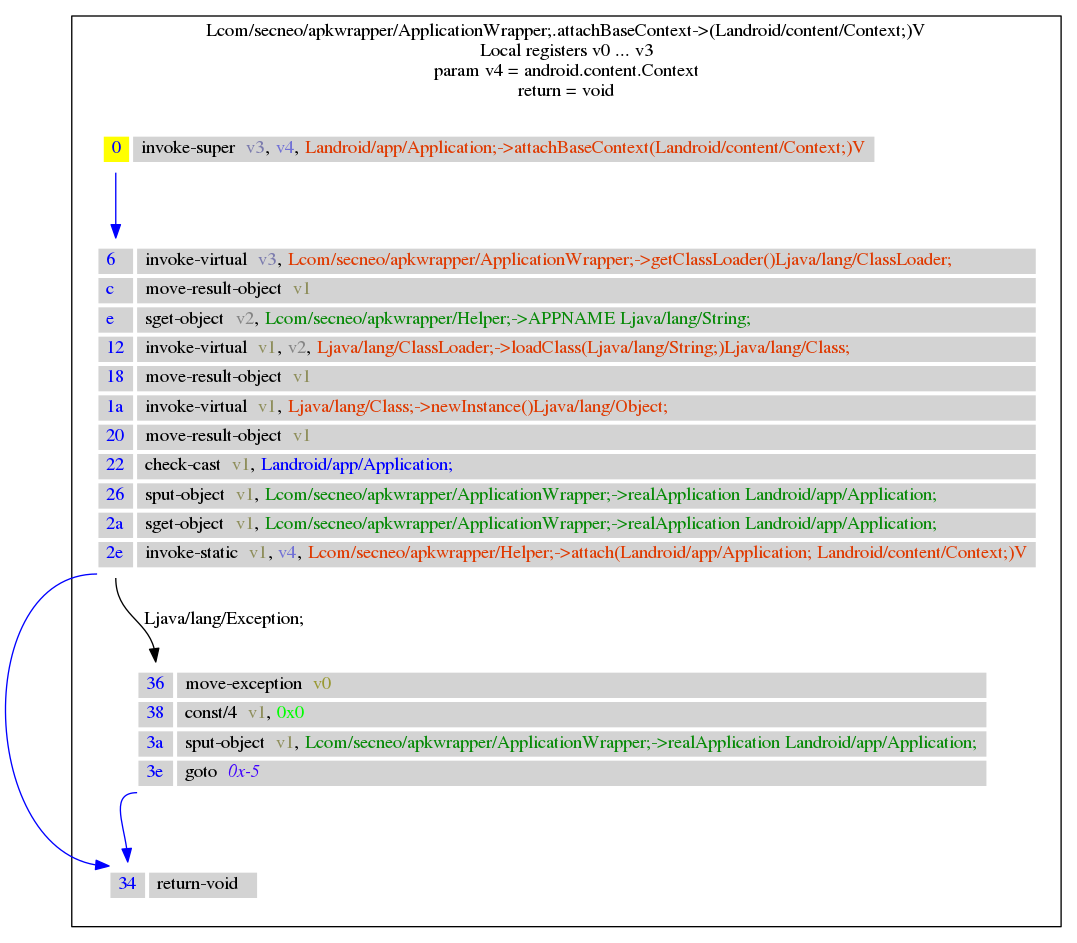
\includegraphics[width=8cm] {cfgexample.png}}
  \caption{An example of a method CFG in a real apk}
\end{figure}

 
\section{An example of 5UD-CFG embedding}
we give an example to show how to calculate $\omega_i$. As shown in the Fig. 2 , vertex $A$ with the first sequence number is called by the vertex $B$ and the vertex $C$ directly. The vertex $C$ is called by the vertex $D$ directly, and vertex $D$ is called by the vertex $E$ directly. This outgoing degree of vertex $A$ is $A_{\searrow B}^{\nearrow C \longrightarrow D \longrightarrow E}$. $A$ is related with $B$, $C$, $D$ and $E$. The result of vertex $A$ will be passed to vertex $B$ and vertex $C$, which have a first-order call structure with vertex $A$. This process will also influence the vertex $D$ and $E$ by influencing the vertex $C$, which are the second-order call structure. 
%\begin{figure}[hbt]
%  \center{\includegraphics[width=8cm] {cfg.eps}}
%  \caption{\label{1}  An example of real CFG}
%\end{figure}

Based on the above first-order call structure and the second-order call structure, the particular trained process of $W$ is as follows:

\begin{eqnarray*}
	\begin{cases}
		\frac{\partial~Link_1^{(1)}}{\partial~\omega_1} +\frac{\partial~Link_2^{(1)}}{\partial~\omega_1}=0\\
		\frac{\partial~Link_1^{(2)}}{\partial~\omega_2} +\frac{\partial~Link_2^{(2)}}{\partial~\omega_2}=0\\
		\frac{\partial~Link_1^{(3)}}{\partial~\omega_3} +\frac{\partial~Link_2^{(3)}}{\partial~\omega_3}=0\\
		\frac{\partial~Link_1^{(4)}}{\partial~\omega_4} +\frac{\partial~Link_2^{(4)}}{\partial~\omega_4}=0\\
		\frac{\partial~Link_1^{(5)}}{\partial~\omega_5} +\frac{\partial~Link_2^{(5)}}{\partial~\omega_5}=0.\\
		%\omega=4+0+2+1+0=7.
	\end{cases}
\end{eqnarray*}

let $log(1+exp \left\{ k\times \omega_i \times \omega_j \right\} )=k\times \omega_i \times \omega_j$ and the weight of final vertex $\omega_5=0$, we have
\begin{eqnarray*}
	\begin{cases}
		9\omega_2+10\omega_4+6\omega_5=0 \\
		35\omega_3+37\omega_4+18\omega_5-18\omega_1=0 \\
		20\omega_5+35\omega_2-18\omega_1=0 \\
		25\omega_5+37\omega_2+10\omega_1-60\omega_3=0 \\
		20\omega_3+6\omega_1+18\omega_2-50\omega_4=0 \\
		W={\omega_1, \omega_2,\omega_3,\omega_4,\omega_5 }~mod~4.
	\end{cases}
\end{eqnarray*}

We obtain the $W=[1,~2,~3,~1,~0].$

 Based on the Definition 6, we calculate the feature of a 5UD-CFG as follows:
\begin{eqnarray*}
	\begin{cases}
	    \omega=1+2+3+1+0=7. \\
		f_n=\frac{1\times 2\times 1+ 2\times 1\times 2+3\times 2\times3+ 4\times 2\times 1 +5\times 1 \times 0}{1+2+3+1+0}=4.57\\
		f_s=\frac{1\times 2\times 1+ 7\times 1\times 2+4\times 2\times3+ 4\times 2\times 1 +1\times 1 \times 0}{1+2+3+1+0}=6.857\\
		f_i=\frac{0\times 2\times 1+ 1\times 1\times 2+1\times 2\times3+ 1\times 2\times 1 +1\times 1 \times 0}{1+2+3+1+0}=1.429\\
		f_o=\frac{0\times 2\times 1+ 2\times 1\times 2+1\times 2\times3+ 1\times 2\times 1 +0\times 1 \times 0}{1+2+3+1+0}=1.714\\
		f_l=\frac{0\times 2\times 1+ 0\times 1\times 0+0\times 2\times2+ 0\times 2\times 1 +0\times 1 \times 0}{1+2+3+1+0}=0.\\
		
	\end{cases}
\end{eqnarray*}

\begin{figure}[hbt]
  \center{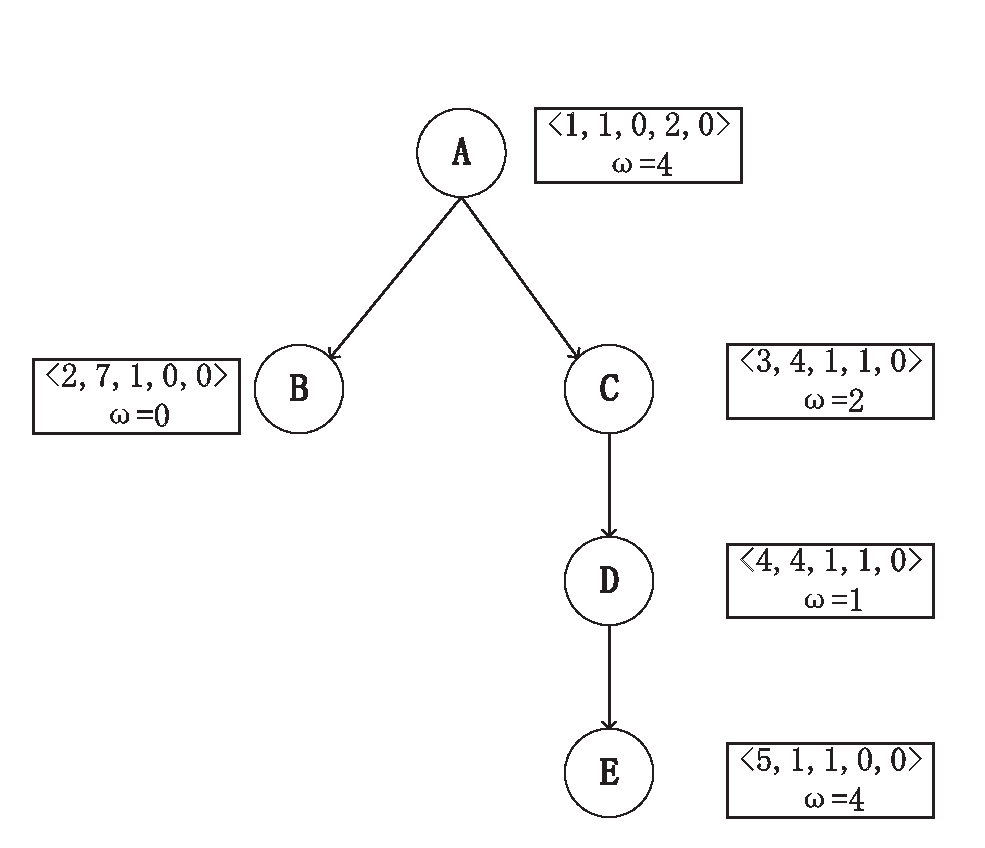
\includegraphics[width=8cm] {feature.eps}}
  \caption{\label{1}  An example of CFG with embedding parameters}
\end{figure}

\section{Evolution compared approaches}
We prepare three representative app clone analysis or bug search techniques to compare our evaluation: Binary search based the Centroid, Gemini based Neural Network, Genius. We introduce the main idea for these three solutions as follows:
\begin{enumerate}
  \item \textbf{Centroid:} The centroid-based approach shows the scalability and accuracy for the app clone. We implemented a centroid bug search method for the five markets. This paper used a geometry characteristic, centroid, of dependency graphs to measure the similarity between methods in two apps.
  \item \textbf{Gemini:} Gemini shows a novel neural network-based approach to compute the embedding based on the control flow graph of each binary function. We set the same iteration number of neural network as $5$. According to the proposed method by this paper, we use the above five datasets to train the embedding database.

  \item \textbf{Genius:} Genius is a bug search system based on the CFG, which can scalable search bugs in the cross-platform. Genius's source code is not available. We use the proposed method to generate $16$ codebooks, and then complete the search database. We compare accuracy and efficiency with our method.  
\end{enumerate}






 